\documentclass[letter,11pt]{article}
\usepackage{latexsym}
\usepackage{xcolor}
\usepackage{float}
\usepackage{amsthm}
\usepackage{amssymb}
\usepackage{wrapfig}
\usepackage{tabularx}
\usepackage{titlesec}
\usepackage{tikz}
\usepackage{geometry}
\usepackage{verbatim}
\usepackage{enumitem}
\usepackage{fancyhdr}
\usepackage{pgfornament}
\usepackage{multicol}
\usepackage{graphicx}
%\usepackage{cfr-lm}
\usepackage{booktabs}
\usepackage{svg}
\usepackage[T1]{fontenc}
\usetikzlibrary{trees}
\setlength{\multicolsep}{0pt} 
\pagestyle{fancy}
%\fancyhf{} % clear all header and footer fields
\fancyhead{}\fancyfoot{}
\fancyhead[R]{\textbf{\thepage}}
\fancyhead[L]{Aiden M. Rosenberg, MMXXIII A.D. }
\addtolength{\headwidth}{3cm}

\usepackage{pgfplots}
\pgfplotsset{compat=1.17}


\renewcommand{\headrulewidth}{1pt}
\renewcommand{\footrulewidth}{0pt}
\geometry{left=1.5cm, top=2.5cm, right=1.5cm, bottom=2cm}

%\usepackage{draftwatermark}	
%\SetWatermarkColor[gray]{0.9}
%\SetWatermarkText{Private}
%\SetWatermarkScale{3}

\usepackage[most]{tcolorbox}
\tcbset{
	frame code={}
	center title,
	left=0pt,
	right=0pt,
	top=0pt,
	bottom=0pt,
	colback=gray!20,
	colframe=white,
	width=\dimexpr\textwidth\relax,
	enlarge left by=-2mm,
	boxsep=4pt,
	arc=0pt,outer arc=0pt,
}


\raggedright
\setlength{\tabcolsep}{0in}

% Sections formatting
\titleformat{\section}{
  \vspace{-4pt}\scshape\raggedright\large
}{}{0em}{}[\color{black}\titlerule \vspace{-7pt}]

\begin{document}

\thispagestyle{empty}

\fontfamily{cmr}\selectfont
%----------HEADING-----------------

\parbox{2.35cm}{%
  \includesvg[width=2.3cm]{logo.svg}
}
\parbox{0.3cm}{\hspace{0.3cm}}
\parbox{\dimexpr\linewidth-5cm\relax}{
\setlength{\tabcolsep}{0.5em}
\def\arraystretch{1.25}
\begin{tabular}{@{}llll@{}}
\toprule
 \multicolumn{4}{c}
 {\hspace{-0.5em}\textbf{Assignment}: Worksheet \#4 (15.5-15.7)} \\ \midrule
\textbf{Name:}      & D. Aiden M. Rosenberg    & \textbf{Professor:}   & Dr. Alan v. Herrmann Ph.D        \\
\textbf{Course:}    & Calculus III        & \textbf{Date:}        & September 7th, 2023 A.D.   \\ \bottomrule
\end{tabular}
}
\vspace{1cm}

\section*{Section 15.5}
The temperature $T(x, y)$ at points in the $xy-$plane is given by $T(x, y) = x^2 - 2y^2$. If an ant were crawling at a constant speed along the $xy-$plane, find the rate of change of temperature if it moved from $(2, -1)$ in the direction of vector $\vec{v} = -\hat{i} + 2 \hat{j}$.
\begin{enumerate}[label=\roman*.]
    \item $\vec{v} = \langle 2, -1 \rangle \Longrightarrow \vec{u} = \frac{\vec{v}}{|\vec{v}|} =  \frac{\vec{v}}{\sqrt{1^2+2^2}} = \left\langle \frac{2}{\sqrt{5}}, \frac{-1}{\sqrt{5}} \right\rangle$ 
    \item $\nabla T = \langle 2x, -4y \rangle \Longrightarrow \nabla T(2,-1) = \langle 4,4\rangle$
    \item $D_{\vec{u}} T(2,-1) =  \nabla T(2,-1)  \cdot \vec{u} =\left( \frac{2}{\sqrt{5}}\right)(4)+ \left(\frac{-1}{\sqrt{5}}\right)(4) = \frac{4\sqrt{5}}{5}$
\end{enumerate}

\section*{Section 15.5} 
Suppose you are climbing a hill whose shape is given by the equation $f(x,y) =z= 1000 - 0.01x^2 - 0.005y^2$ where $x$, $y$, and $z$ are measured in meters and you are standing above point $P(60, 40)$. The positive $x$-axis points east and the positive $y$-axis points north.
\begin{enumerate}[label = \Alph*.]
    \item Find the vector that gives the direction of steepest ascent (maximum rate of increase) at $P$.
        \begin{enumerate}[label=\roman*.]
            \item $\nabla f(P) = \langle -0.02 x, -0.01y \rangle$
            \item $\nabla f(60,40) = \langle -1.2, -0.4 \rangle$
        \end{enumerate}
    \item Determine the maximum rate of ascent (maximum rate of increase) at $P$.
        \begin{enumerate}[label=\roman*.]
            \item $D_{\vec{u}}f(P) =|\vec{v}f(P)|\cos \theta =\sqrt{(-1.2)^2+(-0.4)^2} \cdot \cos (0) = \frac{2\sqrt{10}}{5}$
        \end{enumerate}
    \item Find the vector that gives the direction of steepest descent (minimum rate of increase) at $P$. 
    \begin{enumerate}[label=\roman*.]
        \item $-\nabla f(60,40) = \langle 1.2, 0.4 \rangle$
    \end{enumerate}
\end{enumerate}
\section*{Section 15.6}
Consider surface $S:z = 12 -3x^2$.
\begin{figure}[h]
	\centering
        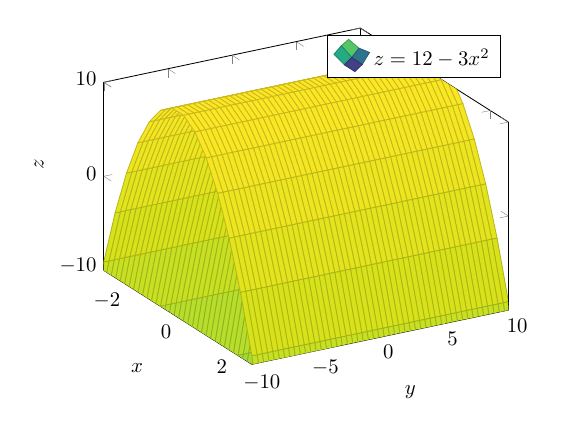
\begin{tikzpicture}[scale = 0.75]
              \begin{axis}[
                    xlabel=$x$,
                    ylabel=$y$,
                    zlabel=$z$,
                    domain=-10:10,
                    y domain=-10:10,
                    zmin=-10,
                    zmax=10,
                    samples=50,
                    colormap/viridis,
                    view={60}{30},
	      			]
                \addplot3[surf] {12 - 3*x^2};
                \addlegendentry{$z = 12 -3x^2$}
              \end{axis}
        \end{tikzpicture}
        \caption{Graph of surface $S$}
        \end{figure}
\begin{enumerate}[label = \Alph*.]
    \item Draw a well-labeled graph of surface $S$.
    \begin{enumerate}[label=\roman*.]
        \item See Figure 1
    \end{enumerate}
    \item Find the equation for the tangent plane to $S$ at point $P (-1, 2, 9)$. Put your answer in simplified $ax + by + cz = d$ format.
    \begin{enumerate}[label=\roman*.]
        \item $F_{x} = -6x$, $F_{y} = 0$, and $F_{z}=-1$
        \item $0=F_{x}(x-x_0)+F_{y}{y-y_0}+F_{z}(z-z_0)$
        \item $0=6(x+1)-1(z-9) = 6x-z+15 \Longrightarrow z = 6x+15$
    \end{enumerate}
    \item Find the linear approximation $L(x, y)$ of $f (x, y) = 12-3x^2$ at $P (-1, 2, 9)$.
    \begin{enumerate}[label=\roman*.]
        \item $L(x,y) = f(x_{0}, y_{0}) + f_{x}(x_0,y_0) (x-x_0)+f_{y}(x_0,y_0)(y-y_0)$
        \item $L(x,y) = 9 + 6(x+1) = 6x+15$
    \end{enumerate}
\end{enumerate}
\section*{Section 15.6}
The length and width of a rectangle are measured as 10 cm and 5 cm respectively. Use the total differential
to determine the maximum error in the calculated area of the rectangle if the error in each measurement is at most 0.05 cm.
\begin{align*}
    A & =L \times W \\
    dA &= \frac{\partial A}{\partial L} \, dL + \frac{\partial A}{\partial W} \, dW \\
    dA &= W \, dL + L\, dW \\
    dA &= 5 \text{ cm} \cdot  0.05 \text{ cm} + 10 \text{ cm} \cdot  0.05 \text{ cm}  = 0.75 \text{ cm}^2\\
\end{align*}


\section*{Section 15.7}
Consider the surface given by the graph of $f (x, y) = 3x^3 + 3y^2 - 6xy - 24y + 15$. Find the $x-$ and $y-$ values where local extrema occur and saddle points occur. Then classify all local extrema and saddle points on this surface using the Second Derivative Test.

\subsection*{Critical Values}
The partial derivatives are given by:
\[
\frac{\partial f}{\partial x} = 9x^2 - 6y \quad \text{and} \quad \frac{\partial f}{\partial y} = 6y - 6x - 24
\]

Setting $\nabla f(x, y) = 0$, we get the following system of equations:
\[
\begin{cases}
9x^2 - 6y = 0 & \text{(1)} \\
6y - 6x - 24 = 0 & \text{(2)}
\end{cases}
\]

Solving equation (1) for $y$:
\[
9x^2 - 6y = 0 \implies y = \frac{9x^2}{6} = \frac{3x^2}{2}
\]

Substituting this into equation (2) and simplifying:
\[
6\left(\frac{3x^2}{2}\right) - 6x - 24 = 0 \implies 9x^2 - 6x - 24 = 0 \implies 3x^2 - 2x - 8 = 0
\]

Applying the quadratic formula ($a = 3$, $b = -2$, $c = -8$):
\[
x = \frac{2 \pm \sqrt{(-2)^2 - 4(3)(-8)}}{2(3)} = \frac{2 \pm \sqrt{4 + 96}}{6} = \frac{2 \pm \sqrt{100}}{6} = \frac{2 \pm 10}{6}
\]

This gives us two critical values for $x$:
\begin{enumerate}
    \item $x_1 = \frac{2 + 10}{6} = \frac{12}{6} = 2$
    \item $x_2 = \frac{2 - 10}{6} = \frac{-8}{6} = -\frac{4}{3}$
\end{enumerate}

Corresponding $y$ values:
\begin{align*}
    \text{For } x = 2, \quad y_1 &= \frac{3(2)^2}{2} = 6 \\
    \text{For } x = -\frac{4}{3}, \quad y_2 &= \frac{3\left(-\frac{4}{3}\right)^2}{2} = \frac{16}{6} = \frac{8}{3}
\end{align*}

The critical points are:
\begin{enumerate}
    \item $(x_1, y_1) = (2, 6)$
    \item $(x_2, y_2) = \left(-\frac{4}{3}, \frac{8}{3}\right)$
\end{enumerate}

\subsection*{Hessian Matrix}

The Hessian matrix is given by:
\[
Hf(x, y) = \begin{bmatrix}
f_{xx} & f_{xy} \\
f_{yx} & f_{yy}
\end{bmatrix}
\]

Where:
\begin{enumerate}[label = \roman*.]
    \item $f_{xx} = 18x$
    \item $f_{yy} = -6$
    \item $f_{xy} = f_{yx} = 6$
\end{enumerate}

For $(x_1, y_1) = (2, 6)$:
\[
Hf(2, 6) = \begin{bmatrix}
36 & 6 \\
6 & -6
\end{bmatrix} = (36)(-6) - (6)(6) = -216 - 36 = -252
\]
Determinant for $Hf(2, 6)$: is is negative, thus critical point corresponds to a saddle point.

For $(x_2, y_2) = \left(-\frac{4}{3}, \frac{8}{3}\right)$:
\[
Hf\left(-\frac{4}{3}, \frac{8}{3}\right) = \begin{bmatrix}
-24 & 6 \\
6 & -6
\end{bmatrix} = (-24)(-6) - (6)(6) = 144 - 36 = 108 
\]


Determinant for $Hf\left(-\frac{4}{3}, \frac{8}{3}\right)$: is is positive, and $f_{xx}$ at $(x_2,y_2)$ is negative, thus critical point corresponds to a local maxima.

\end{document}
